\documentclass[german,oneside,color]{htldipl}
\usepackage{blindtext}
\usepackage[T1]{fontenc}
\usepackage[utf8]{inputenc}
\usepackage{array}
\usepackage{biblatex}
\usepackage{footmisc}

\graphicspath{{images/}}    % Bilderverzeichnis
\usepackage[paper=a4paper,margin=3cm]{geometry}

\makeindex[title=Index]
\makeindex[name=allgemein, title=Allgemeiner Index]
\makeindex[name=name,title={Autoren Index}]
\makeindex[name=title,columns=1,title={Literatur Index}]
\indexsetup{level=\subsection*, toclevel=subsection, noclearpage}


\makeatletter
\@ifpackageloaded{biblatex_legacy}
  {\DeclareIndexNameFormat{default}{%
     \usebibmacro{index:name}{\index[name]}{#1}{#3}{#5}{#7}}}
  {\DeclareIndexNameFormat{default}{%
     \usebibmacro{index:name}{\index[name]}
       {\namepartfamily}
       {\namepartgiven}
       {\namepartprefix}
       {\namepartsuffix}}}
\makeatother

\DeclareIndexFieldFormat{indextitle}{%
  \usebibmacro{index:title}{\index[title]}{#1}}

\renewbibmacro*{bibindex}{%
  \ifbibindex
    {\indexnames{author}%
     \indexnames{editor}%
     \indexnames{translator}%
     \indexnames{commentator}%
     \indexfield{indextitle}}
    {}}

\makeatletter
\DeclareCiteCommand{\repeatfootcite}[\cbx@wrap]
  {\gdef\cbx@keys{}}
  {\xappto\cbx@keys{\thefield{entrykey},}}
  {}
  {\ifcsundef{cbx@lastin@\cbx@keys @\strfield{postnote}}
     {\csnumgdef{cbx@lastin@\cbx@keys @\strfield{postnote}}{-1}}{}%
   \ifsamepage{\value{instcount}}{\csuse{cbx@lastin@\cbx@keys @\strfield{postnote}}}
     {\footnotemark[\csuse{cbx@lastfn@\cbx@keys @\strfield{postnote}}]}
     {\xappto\cbx@cite{\noexpand\footcite%
        [\thefield{prenote}][\thefield{postnote}]{\cbx@keys}%
        \csnumgdef{cbx@lastfn@\cbx@keys @\strfield{postnote}}{\value{\@mpfn}}%
        \csnumgdef{cbx@lastin@\cbx@keys @\strfield{postnote}}{\value{instcount}}}}}

\newrobustcmd{\cbx@wrap}[1]{#1\cbx@cite\gdef\cbx@cite{}}
\def\cbx@cite{}
\makeatother
\addbibresource{literatur.bib}
 
 \newcommand{\putz}
 {\marginpar{\scriptsize{\textit{$\rightarrow$Putz}}}}
 
  \newcommand{\strahlhofer}
 {\marginpar{\scriptsize{\textit{$\rightarrow$Strahlhofer}}}}
 
  \newcommand{\bauer}
 {\marginpar{\scriptsize{\textit{$\rightarrow$Bauer}}}}
 
  \newcommand{\reiter}
 {\marginpar{\scriptsize{\textit{$\rightarrow$Reiter}}}}

\begin{document}

\title{EMS - Event Management Software zum Verwalten und Organisieren von Events jeglicher Art und deren Werbetreibender}
\abteilung{Informatik}
\schwerpunkt{Ausbildungsschwerpunkt Informatik}
\studienort{Wiener Neustadt}
\schule{HTBLuVA Wiener Neustadt}
\schullogo{htl.jpeg}
\abgabejahr{2020/21}
\betreuerA{Dipl.-Ing. Harald Breidler}
\betreuerB{}
\betreuerC{}
\schuelerA{Maurice PUTZ}
\evidenzA{5AHIF-16}
\subthemaA{DSGVO konformes Nutzen von Cloud-Diensten und Gegenüberstellung von Cloud-Computing Anbietern}
\schuelerB{Benjamin STRAHLHOFER}
\evidenzB{5AHIF-20}
\subthemaB{Benjamin Strahlhofer - Subthema}
\schuelerC{Thomas BAUER}
\evidenzC{5AHIF-2}
\subthemaC{Thomas Bauer - Subthema}
\schuelerD{Alexander REITTIER}
\evidenzD{5AHIF-KA}
\subthemaD{Alexander Reiter - Subthema}
\schuelerE{}
\evidenzE{}
\subthemaE{}

%%%----------------------------------------------------------
\frontmatter
\maketitle
\tableofcontents
\listoffigures

%%%----------------------------------------------------------

%Hier kommen die Includes für die Einleitung	
%\chapter{Vorwort}
Dieses Dokument wurde im Rahmen der Reife- und Diplomprüfung 2020/21 an der Höheren Technischen Bundes-, Lehr- und Versuchsanstalt Wiener Neustadt verfasst. Die Idee für dieses Projekt ging von vier engagierten HTL Schülern aus, durch
private Erfahrungen im Management, Marketing und der Organisation betreffend Events und Veranstaltungen. Daraufhin entstand die Idee, mithilfe einer Software viel manuellen Aufwand in der Organisation von Events zu automatisieren. Zuerst zusammen mit einem Unternehmen
welches seine Tätigkeit als Event planer ausführt, wurde die Idee letztendlich von uns vier weiter ausgebaut und realisiert.
Die Software ist bei Release eine individuelle Anwendung, welche später, durch verschiedene Upgrades im allgemeinen lizenziert vergeben werden soll.\newline
Eine maßgeblich daran beteiligte Person und auch Initiator des Unterfangens, konnte die Idee leider nicht mit uns in der Projektgruppe aufgrund gewisse Komplikationen, umsetzen.\newline
Vielen Dank an Herrn Peter Hammer, für seine Ideen und maßgeblich Entscheidende Anfangsidee für so ein Projekt.
Besonderer Dank gilt unserem äußerst engagierten Betreuer, Herrn Prof. Harald Breidler, dass er zu Jahresanfang freiwillig unsere Projektgruppe noch im letzten Moment betreute. Weiters Danken wir herzlich unserem SYP-Lehrer, Herr Prof. Markus Reis
welcher uns im Laufe dieses Projekts jederzeit mit einem gutem Rat zur Seite stand. 
Des Weiteren gilt unseren Familien und Freunden besonderer Dank, die uns in dieser stressigen Zeit viel Kraft gegeben haben. 

%%Inkludiert die 4. vorgeschriebenen Seiten an Dokumentation aus dem gedruckten PDF-Formular
%Das Formular erst vor der Abgabe vollständig ausfüllen, da z.B. das Bild zur Diplomarbeit vorher nicht vorhanden sein wird
\begingroup
\makeatletter
\newpage
\@twosidefalse
\includepdf[pages=1-1,pagecommand={\chapter[Diplomarbeit Dokumentation]{}}]{pdf/Formular-printed.pdf}
\includepdf[pages=2-2,pagecommand={\thispagestyle{plain}}]{pdf/Formular-printed.pdf}
\includepdf[pages=3-3,pagecommand={\chapter[Diploma Thesis Documentation]{}}]{pdf/Formular-printed.pdf}
\includepdf[pages=4-4,pagecommand={\thispagestyle{plain}}]{pdf/Formular-printed.pdf}
\endgroup

%\chapter{Kurzfassung}
Die Software EMS soll in jeder Situation ein professionelles Eventmangement ermöglichen.
Die Kernaufgaben liegen darin, dass Benutzer und Tickets zusammen mit Events verwaltet werden können.
Sogenannte Influencer und Promoter, welche hauptsächlich Personen mit einer großen Reichweite auf Social Media Kanälen sind, ist die neueste Art von Marketing und verspricht für ein Event schnell, viel Aufmerksamkeit zu bekommen.
Diese App soll eine Plattform bieten, diese Influencer und Promoter leicht und überschaulich zu verwalten und das Marketing eines Event dadurch besser zu koordinieren.
Weiters soll durch die Applikation der Eintrittsticketverkauf und der Prozess dahinter, vor allem organisatorisch verbessert und übersichtlicher gemacht werden. 
Die Software unterscheidet einen Benutzer anhand von zwei Rollen, eine Rolle ist die des Promoters, die andere ist die eines Administrators.

Die Anwendung gliedert sich in drei verschiedene Hauptseiten auf, wovon zwei einem normalen Promoter zugänglich sind.
Jeder Promoter hat ein Profil mit seinem Namen, einem Profilbild und einer Beschreibung. Dieses Profil können die Promoter selbst anpassen. Der Name ist jedoch nicht von einem normalen Promoter änderbar.
Die Hauptseite umfasst die Übersicht aller Events. Hier werden alle dem Promoter zugeteilten Events, für welche er Karten verkaufen soll, angezeigt.
Er kann auf eines der Events klicken und gelangt dadurch auf eine detailliertere Seite der gewählten Veranstaltung.
Hier kann er seinen Kartenstand aktualisieren. Für jede verkaufte Karte oder jedes verkaufte Package (Sammlung von Karte) bekommt ein Promoter sogennante Goodie-Punkte.
Diese Punkte kann er dann auf der Event-Details Seite für bestimmte Goodies eintauschen, wie beispielweise \textbf{Ein gratis Getränk beim Event für 10 Punkte}.

Die letzte Seite ist das Admin-Terminal. Wie der Name schon sagt steht diese Seite nur einem Administrator zur Verfügung.
Hier kann dieser einen Benutzer erstellen, ihn deaktivieren und aktivieren und einem Benutzer einem Event zuweißen.
Weiters werden hier auch die Events erstellt indem man Kartentypen, Packages und Belohnungen für die Goodie-Punkte zum einlösen, festlegt.

\textbf{Hinweis:} Sämtliche angegebenen Quellen und Links wurden mit Stand 20.04.2021, 16:00 auf Ihre Richtigkeit und Integrität überprüft.
Sie entsprechen dem momentanen Stand des Wissens in ihren jeweiligen Gebieten zu gegebenem Datum.
Änderungen der Quellen nach angegebenem Zeitpunkt wurden nicht in dieses Dokument übernommen.
Falls solche stattfinden ist das Dokument als veraltet zu betrachten und muss aktualisiert werden.
Die Daten bei den Quellen wurden mithilfe eines selbst erstellten JavaScripts auf ihre aktualität überprüft.
%\include{Abstract}

%%%----------------------------------------------------------
\mainmatter           %Hauptteil (ab hier arab. Seitenzahlen)
%%%----------------------------------------------------------
%\appendix
%Hier kommen die Includes für den Hauptteil
%\chapter{Einleitung}
\section{Ausgangslage}
Bei Veranstaltungen mit einer Alterszielgruppe von 16-21 - jährigen wird heutzutage oft auf Marketing mit Influencer und Promoter gesetzt. 
Sogenannte Influencer und Promoter sind hauptsächlich auf Instagram, Facebook und anderen Social-Media Netzwerken tätig und bewerben dort das jeweilige Event. 
Nachdem eine Nachfrage nach Eintrittskarten besteht, ist es die Aufgabe der Promoter den Eintrittskartenvertrieb zu übernehmen. 
Influencer bewerben weiterhin nur das Event und verkaufen allerdings keine Karten. 
Bei diesen Events müssen 100-150 Promoter Karten erhalten, verkaufen und zu einen späteren Zeitpunkt das eingenommen Geld abgegeben. Dadurch entsteht eine großer 
administrativer Aufwand. Aktuell wird alles mit Hand geführten Protokollen und Listen dokumentiert. Dies sorgt bei dieser Anzahl an Daten schnell für Fehler desen suche
oft viel Zeit in Anspruch nimmt. Für die Auswertung der gesammelten Daten wird eine hochkomplexe Excel Liste benutzt. Leider ist dieser Prozes oft ungenau und wichtige 
Daten gehen verloren oder der Verlauf ist später nicht mehr nachvollziehbar. 

\section{Ziele}
Durch eine iOS und Android App soll den Promoter-Managern und der Eventleitung viel organistorischer Aufwand abgenommen werden. Weiters soll die Fehlerquote stark gesenkt werden
wodurch in manchen Fällen viel Geld gespart werden kann. 

\newpage
\section{Team}
\subsection{Maurice Putz}
\subsubsection{Themenstellung}
Chatsystem in EMS, Cloud Computing und Beispiel eines Backend Deployment in AWS mit Schwerpunkt auf Grundlagen im Datenschutz und DSGVO Konformität
\subsubsection{Rolle}
In diesem Projekt übernahm er die Rolle eines Fullstack Entwickler. Er hatte die Verantwortung für das Chatsystem,
sowie zahlreiche Funktionen im Front- sowie Backend. Außerdem war er für das Deployment des Backend der App am Ende zuständig.

\subsection{Benjamin Strahlhofer}
\subsubsection{Themenstellung}
Anmeldesystem in EMS, Sicherheitsrisiken Abwicklung und Vergleich ein Biometrie, mit dem Schwerpunkt auf Sicherheit eines Anmeldesystems
\subsubsection{Rolle}
In diesem Projekt Übernahm er die Rolle eines Fullstack Entwickler. Er hatte die Verantwortung für das Anmeldesystem und 
sowie zahlreiche Funktionen im Front- und Backend.

\subsection{Thomas Bauer}
\subsubsection{Themenstellung}
Allgemeines zu Data Analytics und Grundlagen von Rest API's, Vergleich von SQL und einer NoSQL Datenbank mit Schwerpunkt auf Datenbankentwurf
\subsubsection{Rolle}
In diesem Projekt Übernahm er die Rolle eines Fullstack Entwickler. Er hatte die Verantwortung über die Datenbank, 
sowie zahlreiche Funktionen im Front- und Backend. 

\subsection{Alexander Reiter}
\subsubsection{Themenstellung}
Ticketsysteme, Untersuchung von Belohnungssystemen für Wettbewerbssituationen und Vorgehensmodelle mit Schwerpunkt auf einem Vergleich von SCRUM und RUP
\subsubsection{Rolle}
JA WAS DENN? HA HA HA? GOR NIX, KONNST NIX, SCHENE GRIAS

\newpage

%ZB
%\include{Grundlagen_Putz}
%\include{Vergleich_Putz}

%%%----------------------------------------------------------
%%%Anhang
%%%----------------------------------------------------------
%\appendix

%%Hier kommen die Includes für den Anhang

%%%----------------------------------------------------------
%Ausgabe der automatischen Zusatzdaten: Glossar, Index, Literaturverzeichnis
%\clearpage
%\printglossaries

\clearpage
\chapter*{Index}
\addcontentsline{toc}{chapter}{Index}
\printindex[allgemein]

\printindex

\printindex[name]

\printindex[title]


%Literaturverzeichnis
\clearpage
\addcontentsline{toc}{chapter}{\bibname}
\printbibliography

\clearpage
\chapter*{Messbox zur Druckkontrolle}



\begin{center}
{\Large --- Druckgröße kontrollieren! ---}

\bigskip

\Messbox{100}{50} % Angabe der Breite/Hoehe in mm

\bigskip

{\Large --- Diese Seite nach dem Druck entfernen! ---}

\end{center}



%%%----------------------------------------------------------
\end{document}